\chapter{Modelling} \label{chp:models}
    Although the work of this project was primarily experimental, some modelling work was performed in order to better understand the physics of LSP and aid in the experimental design. One major area of interest is in determining the absorption properties of LSP. High laser absorption is desirable to maximize power conversion efficiency. Furthermore, the IB absorption coefficient typically reaches a maximum at a specific temperature. According to \textcite{keeferLaserSustainedPlasmas1989}, this peak absorption temperature was found to closely correlate with LSP peak temperature. The measurement of absorption coefficient can thus be used to support LSP temperature estimates.

    \section{Absorption} \label{sec:models_absorption}
        A critical property of LSP is its ability to absorb laser radiation. As stated in \autoref{sec:background_lsp}, the primary mechanism for radiation absorption in LSP is inverse bremsstrahlung. Calculation of the absorption coefficient of this process is critical for modelling LSP behavior and estimating its laser absorption efficiency. The calculation method presented here aims to adapt the work of \textcite{akarapuNumericalModelLasersustained2009,nassarInvestigationLasersustainedPlasma2012}, who have developed CFD models for the use of Argon LSP in surface-treatment applications. Although their work considered \ce{CO_2} lasers, adapting the method to the fiber laser of this study is a matter of using the appropriate laser frequency in \autoref{eq:ib_absorption}. Their work was thus used to validate each calculation step, and their results will be plotted alongside this study's computations when relevant.
        
        The absorption coefficient can be calculated using \autoref{eq:ib_absorption} and is heavily dependent on electron density $n_\mathrm{e}$ and radiation frequency $\nu$. The first step of absorption modelling is thus to determine electron density, which is variable with temperature $T$ according to the Saha ionization equation, developed by \textcite{sahaPhysicalTheoryStellar1997}. It is reproduced here for the single ionization case as \autoref{eq:saha}:
        \begin{equation}
            \frac{n_\mathrm{e}^2}{n_0-n_\mathrm{e}} = \frac{n_\mathrm{e}^2}{n_\mathrm{Ar}} = \frac{2}{\Lambda_\mathrm{th}^3}\frac{\mathcal{Z}_{\mathrm{Ar}^+}}{\mathcal{Z}_\mathrm{Ar}}\exp{\left(-\frac{E_\text{ion, Ar}}{k_\mathrm{B}T}\right)}
            \label{eq:saha}
        \end{equation}
        Where $n_0$ is the initial number density of neutral atoms, $n_\mathrm{Ar}$ is the number density of un-ionized atoms at a given temperature, $E_\text{ion, Ar}$ is Argon's first ionization energy (\qty{15.76}{eV}~\cite{liasIonizationEnergyEvaluation2023}), and $k_\mathrm{B}$ is the Boltzmann constant. The thermal DeBroglie wavelength $\Lambda_\mathrm{th}$ is a function of temperature as follows, where $\hbar$ is the reduced Planck constant and $m_\mathrm{e}$ is the mass of an electron:
        \begin{equation*}
            \Lambda_\mathrm{th} = \sqrt{\frac{2\pi \hbar^2}{m_\mathrm{e}k_\mathrm{B}T}}
        \end{equation*}
        The ratio $\mathcal{Z}_{\mathrm{Ar}^+}/\mathcal{Z}_\mathrm{Ar}$ is the ratio of the partition function values for Ar$^+$ and Ar (also designated Ar II and Ar I, respectively). These values are also dependent on temperature and can be queried in the NIST Atomic Spectra Database (ASD) (\textcite{kramidaNISTAtomicSpectra2022}) for a given spectrum (e.g., Ar I) and electron temperature $T_\mathrm{e}$. This ratio is plotted in \autoref{fig:e_density_partition}. \citeauthor{nassarInvestigationLasersustainedPlasma2012} fitted a seventh-order polynomial (shown in \autoref{eq:nassar_polynomial}) to approximate this ratio across temperature:
        \begin{multline} \label{eq:nassar_polynomial}
            \frac{\mathcal{Z}_{\mathrm{Ar}^+}}{\mathcal{Z}_\mathrm{Ar}} = -2.3077\times 10^{-29}T^7+2.3474\times 10^{-24}T^6 - 8.8453\times 10^{-20}T^5 \\
            + 1.4851\times 10^{-15}T^4 -9.843\times 10^{-12}T^3 - 1.2477\times 10^{-8}T^2 \\
            + 0.00047534T+3.7971
        \end{multline}
        This approximation is plotted alongside the data directly retrieved from the NIST ASD in \autoref{fig:e_density_partition} for comparison.

        It is important to note that $n_0$ in \autoref{eq:saha} is not constant across temperatures. In the case of LSP, the ionization process occurs at constant pressure, even if the experiment occurs in a closed container, as only a small fraction of the test section volume undergoes ionization. The hotter Argon is free to expand into the cooler surroundings, locally reducing the number density and maintaining a constant pressure. Therefore, $n_0$ must be calculated based on a given pressure $p$ and the varying temperature. This can be done with the ideal gas equation, where $V$ is volume, $N$ is the number of atoms in moles, $R_\mathrm{u}$ is the universal gas constant, and $N_\mathrm{A}$ is Avogadro's number:
        \begin{align*}
            pV&= NR_\mathrm{u}T \\
            p&= \frac{N}{V}R_\mathrm{u}T \\
            \frac{N_\mathrm{A}p}{R_\mathrm{u}T}&= n_0
        \end{align*}

        The electron density $n_\mathrm{e}$ is plotted against temperature in \autoref{fig:e_density_curves}, for a pressure of \qty{1}{bar}. The calculation by \citeauthor{nassarInvestigationLasersustainedPlasma2012} is plotted alongside it, and their relative value is compared. While the electron density plots appear to agree, there remains a difference in density of a factor of two. This appears to be due to the use of lower precision physical constants in \citeauthor{akarapuNumericalModelLasersustained2009} and \citeauthor{nassarInvestigationLasersustainedPlasma2012}'s work.

        \begin{figure}[h]
            \centering
            \begin{subfigure}[t]{2.6in}
                \centering
                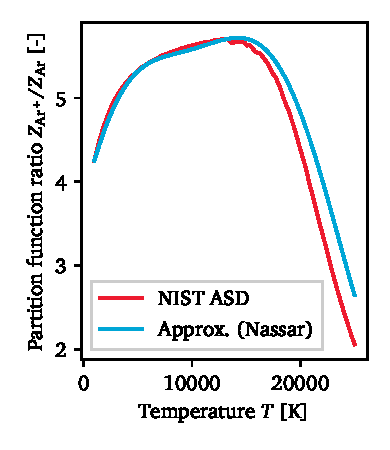
\includegraphics[]{assets/4 models/partition}
                \caption{Ratio of Ar II to Ar I partition function values}
                \label{fig:e_density_partition}
            \end{subfigure}
            \hfill
            \begin{subfigure}[t]{3.2in}
                \centering
                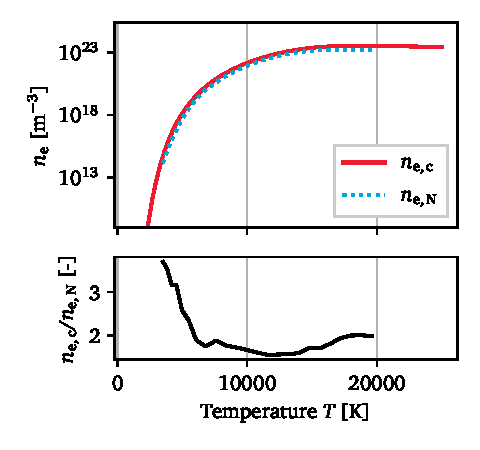
\includegraphics[]{assets/4 models/n_e}
                \caption{$n_\mathrm{e}$ at \qty{1}{bar}, and comparison between computed density $n_\mathrm{e, c}$ and density $n_\mathrm{e, N}$ reported by \textcite{nassarInvestigationLasersustainedPlasma2012}}
                \label{fig:e_density_curves}
            \end{subfigure}
            \caption{Computation of electron density $n_\mathrm{e}$ of Argon}
            \label{fig:e_density}
        \end{figure}

        Although electron density appears to plateau past \qty{20000}{K}, the caveat of this calculation is that it only considers single-ionization. While this is valid below \qty{20000}{K}, second-degree ionization begins past this temperature. The plot is extended up to \qty{25000}{K} to provide some estimate of plasma properties, although they will not be as accurate as below \qty{20000}{K}.

        The absorption coefficient $\alpha$ can now be calculated with the known electron density. For convenience, the equation for $\alpha$, \autoref{eq:ib_absorption}, is reproduced here:
        \begin{equation*}
            \ibalphaeq \tag{\ref{eq:ib_absorption} revisited}
        \end{equation*}
        Most parameters have been defined in \autoref{sec:background_lsp}, so the Coulomb logarithm $\ln{\Lambda}$ and the plasma frequency $\nu_\mathrm{p}$ will be of interest here. The Coulomb logarithm is evaluated by \textcite{nassarInvestigationLasersustainedPlasma2012} using a common approximation seen in plasma physics (\textcite{richardson2019NRLPlasma2019}):
        \begin{equation}\label{eq:coulombLog_NRL}
            \ln{\Lambda} \approx 23-\ln{(n_\mathrm{e}^{1/2}ZT_\mathrm{e}^{-3/2})}
        \end{equation}
        However, alternate evaluations of the logarithm exist, such as the one given by \textcite{johnstonCorrectValuesHighfrequency1973} in the specific context of IB absorption coefficient calculation (\autoref{eq:coulombLog_johnston}). 
        \begin{equation} \label{eq:coulombLog_johnston}
            \Lambda(\nu) = \begin{cases}
                \frac{v_T}{\nu\rho_\mathrm{min}} & \nu \gg \nu_\mathrm{p}\\
                \frac{v_T}{\nu_\mathrm{p}\rho_\mathrm{min}} & \text{otherwise}
            \end{cases}
        \end{equation}
        Where $v_T$ is the electron thermal velocity, $\nu$ is the laser frequency, $\nu_\mathrm{p}$ is the plasma frequency, and $\rho_\mathrm{min}$ is the impact parameter. These can be evaluated with the following equations:
        \begin{gather}
            v_T = \sqrt{\frac{k_\mathrm{B}T}{m_\mathrm{e}}} \\
            \nu_\mathrm{p} = \frac{1}{2\pi}\sqrt{\frac{e^2n_\mathrm{e}}{\epsilon_0 m_\mathrm{e}}} \approx (\qty{8.97885}{m^{3/2}s^{-1}})\sqrt{n_\mathrm{e}}\\
            \rho_\mathrm{min} \approx \max{\left(\frac{Ze^2}{k_\mathrm{B}T}, \frac{\hbar}{(m_\mathrm{e}k_\mathrm{B}T)^{1/2}}\right)}
        \end{gather}
        \textcite{johnstonCorrectValuesHighfrequency1973} state:
        \begin{quote}
            ...at frequencies well above the plasma frequency $\nu_\mathrm{p}$, $\ln{\Lambda}(\nu)$ should contain the wave frequency $\nu$ rather than the plasma frequency $\nu_\mathrm{p}$.
        \end{quote}
        The respective frequencies of the plasma, \ce{CO_2} laser, and fiber laser are plotted in \autoref{fig:coulomb_freq} for comparison. It can be seen that for a fiber-laser-powered LSP, the $\nu \gg \nu_\mathrm{p}$ case of \autoref{eq:coulombLog_johnston} is valid across the range of temperatures of interest, so \citeauthor{johnstonCorrectValuesHighfrequency1973}'s statement is highly relevant in this case, and perhaps of lesser importance in \citeauthor{nassarInvestigationLasersustainedPlasma2012}'s study. Furthermore, the fiber laser frequency is so much greater than the plasma frequency that $(1-\nu_\mathrm{p}^2/\nu^2)^{-1/2} \approx 1$ in \autoref{eq:ib_absorption}. As it was not clear whether the approximation of $\ln{\Lambda}$ in \autoref{eq:coulombLog_NRL} was applicable in this case, both evaluations of the Coulomb logarithm were compared in \autoref{fig:coulomb_coulomb}, showing that while there is a large divergence at lower temperatures, this is negligible as the Argon is not in a plasma state. For temperatures of interest, namely above \qty{10000}{K}, both evaluations of the Coulomb logarithm appear to converge. \citeauthor{johnstonCorrectValuesHighfrequency1973}'s form of the logarithm was retained for further calculations as it considers the relative values of the plasma and laser frequencies.

        \begin{figure}[h]
            \centering
            \begin{subfigure}[t]{2.9in}
                \centering
                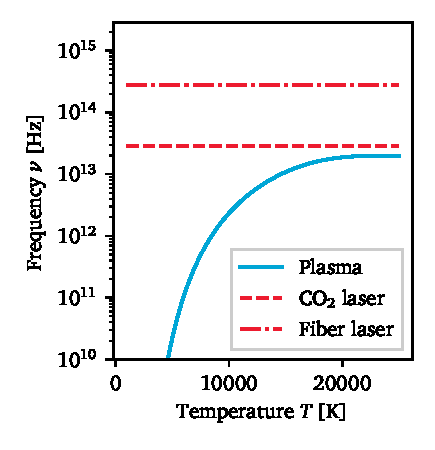
\includegraphics[]{assets/4 models/frequency_comparison}
                \caption{Comparison of plasma and laser frequencies}
                \label{fig:coulomb_freq}
            \end{subfigure}
            \hfill
            \begin{subfigure}[t]{2.9in}
                \centering
                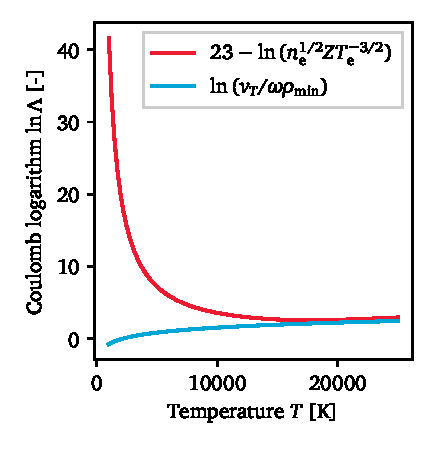
\includegraphics[]{assets/4 models/coulombLog}
                \caption{Comparison of computation methods}
                \label{fig:coulomb_coulomb}
            \end{subfigure}
            \caption{Calculation of the Coulomb logarithm, \qty{10}{bar}}
            \label{fig:coulomb}
        \end{figure}

        With values for the Coulomb logarithm and the plasma frequency, \autoref{eq:ib_absorption} can be evaluated. \autoref{fig:ib_coeff} plots the IB absorption coefficient for a range of temperatures and pressures. The point of peak absorption appears around the \qty{20000}{K} mark, with a sharp rise in peak absorption coefficient with increasing pressure. This is expected as $\alpha$ is proportional to $n_\mathrm{e}^2$ on the first order, which increases with pressure. The occurrence of peak absorption appears to shift to greater temperatures as pressure increases.

        \begin{figure}[h]
            \centering
            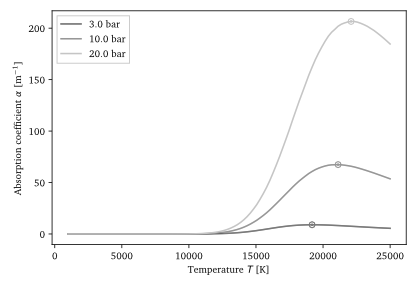
\includegraphics[]{assets/4 models/absorption}
            \caption{Inverse bremsstrahlung absorption coefficient of Argon at various pressures, \qty{1070}{nm} radiation}
            \label{fig:ib_coeff}
        \end{figure}

        The temperature of peak absorption is of interest, as it correlates to the peak temperature of the LSP (\textcite{keeferLaserSustainedPlasmas1989}). This absorption model thus suggests that a peak temperature of around \qty{20000}{K} should be expected.